% @author Adriano
% @date Sat Oct 22 12:57:28 CEST 2016
%-------------------------------------------------------------------------------
% Copyright (c) 2013-2015 University of Luxembourg.
% All rights reserved. This program and the accompanying materials
% are made available under the terms of the Eclipse Public License v1.0
% which accompanies this distribution, and is available at
% http://www.eclipse.org/legal/epl-v10.html
% 
% Contributors:
%     Alfredo Capozucca - initial API and implementation
%     Benoît Ries - minor updates
%     Nicolas Guelfi - most content from messirbook
%--------------------------------------------------------------------------
%%%%%%%%%%%%%%%%%%%%%%%%%%%%%%%%%%%%%%%%%%%%%%%%%%
\PassOptionsToPackage{usenames,svgnames,table}{xcolor}
\documentclass[graybox,envcountchap,sectrefs,11pt]{book}  
%%%%%%%%%%%%%%%%%%%%%%%%%%%%%%%%%%%%%%%%%%%%%%%%%%
%%% DO NOT CHANGE THE ORDER
\usepackage{./../lu.uni.lassy.excalibur.standard.report.libraries/styles/style-messir-common}
\usepackage{./../lu.uni.lassy.excalibur.standard.report.libraries/styles/style-messir-report-post}
%--------------------------------------------
% DOCUMENT BEGIN
%--------------------------------------------
\begin{document}

\newgeometry{textwidth=17cm,textheight=23.7cm} 
 
\newcommand{\msrReportType}{\emph{Report type: Default}~} 



\definecolor{lightgray}{RGB}{201,201,201}
\definecolor{lightred}{RGB}{250,112,97}
\definecolor{lightgreen}{RGB}{179,250,140}

\definecolor{msrtextcl}{RGB}{0,0,0}
\definecolor{msrkeycl}{RGB}{127,0,85}
\definecolor{msrcmtcl}{RGB}{201,201,201}
\definecolor{keywordcolor}{RGB}{30,144,255}

\definecolor{aqua_blue}{RGB}{0,139,145}
\definecolor{dark_green}{RGB}{0,128,0}
\definecolor{dark_blue}{RGB}{45,45,138}

\definecolor{msrcolor01}{rgb}{0.96,0.59,0.48}
\definecolor{msrcolor02}{rgb}{1.00,0.97,0.60}
\definecolor{msrcolor03}{rgb}{0.51,0.79,0.61}
\definecolor{msrcolor04}{rgb}{0.43,0.81,0.96}
\definecolor{msrcolor05}{rgb}{0.52,0.58,0.79}
\definecolor{msrcolor06}{rgb}{0.96,0.61,0.76}
\definecolor{msrcolor07}{rgb}{0.98,0.68,0.51}
\definecolor{msrcolor08}{rgb}{0.77,0.88,0.61}
\definecolor{msrcolor09}{rgb}{0.49,0.66,0.85}
\definecolor{msrcolor10}{rgb}{0.96,0.60,0.62}
\definecolor{msrcolor11}{rgb}{0.64,0.83,0.61}
\definecolor{msrcolor12}{rgb}{0.63,0.53,0.75}
\definecolor{msrcolor13}{rgb}{0.99,0.78,0.54}
\definecolor{msrcolor14}{rgb}{0.53,0.51,0.74}
\definecolor{msrcolor15}{rgb}{0.48,0.80,0.79}
\definecolor{msrcolor16}{rgb}{0.74,0.55,0.75}
\definecolor{msrcolor17}{rgb}{0.90,0.79,0.08}
\definecolor{msrcolor18}{rgb}{1.00,1.00,0.00}
\definecolor{msrcolor19}{rgb}{1.00,0.00,0.50}

\definecolor{sepcolor000000}{rgb}{0, 0, 0}
\definecolor{sepcolor101010}{rgb}{0.10, 0.10, 0.10}
\definecolor{sepcolor202020}{rgb}{0.20, 0.20, 0.20}
\definecolor{sepcolor303030}{rgb}{0.30, 0.30, 0.30}
\definecolor{sepcolor404040}{rgb}{0.10, 0.10, 0.10}
\definecolor{sepcolor505050}{rgb}{0,1,.5}
\definecolor{sepcolor907908}{rgb}{0,1,.5}

\definecolor{sepregioncolor01}{rgb}{0.00,0.66,0.00}
\definecolor{sepregioncolor02}{rgb}{1.00,1.00,0.00}
\definecolor{sepregioncolor03}{rgb}{1.00,0.97,0.60}
\definecolor{sepregioncolor04}{rgb}{0.64,0.83,0.61}
\definecolor{sepregioncolor05}{rgb}{0.95,0.36,0.00}
\definecolor{sepregioncolor06}{rgb}{0.90,0.79,0.08}
\definecolor{sepregioncolor07}{rgb}{0.63,0.53,0.75}
\definecolor{sepregioncolor08}{rgb}{0.99,0.78,0.54}
\definecolor{sepregioncolor09}{rgb}{0.96,0.61,0.76}
\definecolor{sepregioncolor10}{rgb}{1.00,0.00,0.50}

\colorlet{msrcolorbrown}{red!40!black!80}


% Messir General
%----------------------------------------------------------

% quotePosition + quoteWidth + quotefillColor + quoteElement + quotedElement + allImageScale
\newcommand{\msrcallouted}[6]{
\scalebox{#1}{\parbox{\linewidth}{
  \begin{tikzpicture}
      \node [rectangle callout,callout relative pointer={#4},text width=#5,fill=#6,rounded corners] (tmpcall) at (0,0) {#3};
      \node at (tmpcall.pointer){#2};
  \end{tikzpicture}
}}
}

% Vresion wihtout scaling the quoted text
\pgfkeys{%
    /calloutquote/.cd,
    width/.code                   =  {\def\calloutquotewidth{#1}},
    position/.code                =  {\def\calloutquotepos{#1}}, 
    author/.code                  =  {\def\calloutquoteauthor{#1}},
    /calloutquote/.unknown/.code   =  {\let\searchname=\pgfkeyscurrentname
                                 \pgfkeysalso{\searchname/.try=#1,
    /tikz/\searchname/.retry=#1},\pgfkeysalso{\searchname/.try=#1,
                                  /pgf/\searchname/.retry=#1}}
                            }  

\newcommand\calloutquote[2][]{%
  \pgfqkeys{/calloutquote}{#1}
  \node [rectangle callout,callout relative pointer={\calloutquotepos},text width=\calloutquotewidth,/calloutquote/.cd,#1] (tmpcall) at (0,0) {#2};
  \node at (tmpcall.pointer){\calloutquoteauthor};    
}  
%----------------------------------------------------------
\newcommand{\msrTalkRD}[6]{
\freeblock{5}{#1}{#2}{
\begin{figure}
  \centering
  \includegraphics[width=#5]{images/various/descartes.pdf} 
\end{figure}
}
\freeblock{5}{#3}{#4}{
\scriptsize
\textit{#6}
}
}
\newcommand{\msrTalkGB}[6]{
\freeblock{5}{#1}{#2}{
\begin{figure}
  \centering
  \includegraphics[width=#5]{images/various/graham-bell.pdf} 
\end{figure}
}
\freeblock{5}{#3}{#4}{
\scriptsize
\textit{#6}
}
}
%----------------------------------------------------------

\newcommand{\msrQuestionSlide}[1]{
\begin{frame}[fragile]
\freeblock{5}{1}{4}{
\begin{figure}
  \centering
  \includegraphics[width=3cm]{images/various/3d-man-question-sit.pdf}
\end{figure}
}
\freeblock{10}{5}{3}{
\Large
\msrtxtclb{red}{\textit{#1}}
}
\end{frame}
}

%%%%%%%%%%%%%%%%%%%%%%%%%%%%%%%%%%%%%%%%%%%%%%%%%%

\DeclareRobustCommand{\msrfigure}[4]{
\begin{figure}[htbp]
%\centering
\scalebox{#1}{
{\begin{minipage}[c]{\linewidth}
\centering
#2
\end{minipage}
}}
\ifthenelse{\equal{#4}{}}
             {}
             {\caption{#4}}
\label{#3}
\end{figure}
}

\newcommand{\semitransp}[2][30]{\color{fg!#1}#2}
\newcommand*{\msrtechfont}{\fontfamily{ptm}\selectfont}

\DeclareRobustCommand{\msruml}{{\msrtechfont UML}~}
\DeclareRobustCommand{\msrocl}{{\msrtechfont OCL}~}
\DeclareRobustCommand{\msromg}{{\msrtechfont OMG}~}
\DeclareRobustCommand{\msrxtext}{{\msrtechfont Xtext}~}
\DeclareRobustCommand{\msremf}{{\msrtechfont EMF}~}
\DeclareRobustCommand{\msrcm}{\msrcode{{Concept Model}}~}

\DeclareRobustCommand{\msrapache}{{\msrtechfont Apache}~}
\DeclareRobustCommand{\msratlassian}{{\msrtechfont Atlassian}~}
\DeclareRobustCommand{\msrbamboo}{{\msrtechfont Bamboo}~}
\DeclareRobustCommand{\msrconfluence}{{\msrtechfont Confluence}~}
\DeclareRobustCommand{\msreclemma}{{\msrtechfont EclEmma}~}
\DeclareRobustCommand{\msreclipse}{{\msrtechfont Eclipse}~}
\DeclareRobustCommand{\msrsql}{{\msrtechfont SQL}~}
\DeclareRobustCommand{\msrjava}{{\msrtechfont Java}~}
\DeclareRobustCommand{\msrjavafx}{{\msrtechfont JavaFx}~}
\DeclareRobustCommand{\msrjira}{{\msrtechfont JIRA}~}
\DeclareRobustCommand{\msrjunit}{{\msrtechfont JUnit}~}
\DeclareRobustCommand{\msrlatex}{{\msrtechfont Latex}~}
\DeclareRobustCommand{\msrmaven}{{\msrtechfont Maven}~}
\DeclareRobustCommand{\msrmysql}{{\msrtechfont MySQL}~}
\DeclareRobustCommand{\msrocl}{{\msrtechfont OCL}~}
\DeclareRobustCommand{\msrpdf}{{\msrtechfont PDF}~} 
\DeclareRobustCommand{\msrsirius}{{\msrtechfont Sirius}~} 
\DeclareRobustCommand{\msrsvn}{{\msrtechfont SubVersioN}~}
\DeclareRobustCommand{\msrswtbot}{{\msrtechfont SWTbot}~}
\DeclareRobustCommand{\msrxtext}{{\msrtechfont Xtext}~} 

 
\DeclareRobustCommand{\msrmessirmeth}{{\msrmessir}~methodology~}
\newcommand{\msrglsstyle}[1]{\emph{#1}}
\DeclareRobustCommand{\msrucname}[1]{\msrcode{\underline{#1}}}

% Verify macro since creates .toc errors
%\DeclareRobustCommand{\msrcode}[1]{{\normalfont\fontfamily{pcrr}\selectfont #1}}
%\DeclareRobustCommand{\msrcode}[1]{{\normalfont\fontfamily{cmvtt}\selectfont #1}}
\DeclareRobustCommand{\msrcode}[1]{{\protect\ \ttfamily \hyphenchar\font=`\- #1}}

% Messir Lexique
\DeclareRobustCommand{\msrbool}{\msrcode{{\emph Boolean}}~}
\DeclareRobustCommand{\msrint}{\msrcode{{\emph Integer}}~}
\DeclareRobustCommand{\msrreal}{\msrcode{{\emph Real}}~}
\DeclareRobustCommand{\msrstring}{\msrcode{{\emph String}}~}
\DeclareRobustCommand{\msrenum}{\msrcode{{\emph enumeration}}~}
\DeclareRobustCommand{\msrenums}{\msrcode{{\emph enumerations}}~}

% Messir Analysis
\DeclareRobustCommand{\msrsysop}{\emph{system operation}}
\DeclareRobustCommand{\msrsysops}{\emph{system operations}}
\DeclareRobustCommand{\msrsysintpro}{\emph{system interaction protocol}}
\DeclareRobustCommand{\msrbhvmd}{\emph{system operation}}

\newcommand{\msrt}[1]{\textuncl{#1}~}

\DeclareRobustCommand{\msrfont}[1]{\textuncl{#1}}
\DeclareRobustCommand{\msrfontb}[1]{\msrfont{\textbf{#1}}}
\DeclareRobustCommand{\msrfontcl}[1]{\msrfont{{\color{MediumPurple}#1}}}
\DeclareRobustCommand{\msrfontclb}[1]{{\msrfontcl{\textbf{#1}}}}

\DeclareRobustCommand{\msrcl}[1]{{\color{MediumPurple}#1}~}
\DeclareRobustCommand{\msrclb}[1]{{\msrcl{\textbf{#1}}}}

\DeclareRobustCommand{\msrmessir}{\msrfont{Messir}~}
\DeclareRobustCommand{\msrmessirb}{\msrfont{\textbf{Messir}}}
\DeclareRobustCommand{\msrmessircl}{{\color{MediumPurple}\msrmessir}}
\DeclareRobustCommand{\msrmessirclb}{{\color{MediumPurple}\msrmessirb}}

\DeclareRobustCommand{\msrexcalibur}{{\unclfamily Excalibur}~}
\DeclareRobustCommand{\msrexcaliburb}{\msrfont{\textbf{\msrexcalibur}}}
\DeclareRobustCommand{\msrexcaliburcl}{\msrfontcl{\msrexcalibur}}
\DeclareRobustCommand{\msrexcaliburclb}{\msrfontclb{\msrexcalibur}}

\DeclareRobustCommand{\msrmessim}{\msrfont{MesSim}}
\DeclareRobustCommand{\msrmessimb}{\msrfontb{MesSim}}
\DeclareRobustCommand{\msrmessimcl}{\msrfontcl{MesSim}}
\DeclareRobustCommand{\msrmessimclb}{\msrfontclb{MesSim}}

\DeclareRobustCommand{\msrmessam}{\msrfont{MesSam}}
\DeclareRobustCommand{\msrmessamb}{\msrfontb{MesSam}}
\DeclareRobustCommand{\msrmessamcl}{\msrfontcl{MesSam}}
\DeclareRobustCommand{\msrmessamclb}{\msrfontclb{MesSam}}

\DeclareRobustCommand{\msrmevop}{\msrfont{MevoP}~}
\DeclareRobustCommand{\msrmevopb}{\msrfontb{MevoP}~}
\DeclareRobustCommand{\msrmevopcl}{\msrfontcl{MevoP}~}
\DeclareRobustCommand{\msrmevopclb}{\msrfontclb{MevoP}~}

\DeclareRobustCommand{\msrmessep}{\msrfont{Messep}~}
\DeclareRobustCommand{\msrmessepb}{\msrfontb{Messep}~}
\DeclareRobustCommand{\msrmessepcl}{\msrfontcl{Messep}~}
\DeclareRobustCommand{\msrmessepclb}{\msrfontclb{Messep}~}

\DeclareRobustCommand{\msrmessee}{\msrfont{MesSEE}~}
\DeclareRobustCommand{\msrmesseeb}{\msrfontb{MesSEE}~}
\DeclareRobustCommand{\msrmesseecl}{\msrfontcl{MesSEE}~}
\DeclareRobustCommand{\msrmesseeclb}{\msrfontclb{MesSEE}~}

\DeclareRobustCommand{\msrprolog}{{\msrtechfont Prolog}}
\DeclareRobustCommand{\msrmessimb}{\textbf{\msrmessim}}
\DeclareRobustCommand{\msrprologcl}{\textcolor{red}{\msrprolog}}
\DeclareRobustCommand{\msrprologclb}{\textbf{\msrprologcl}}

\DeclareRobustCommand{\msrmcl}{{\footnotesize \msrfont{mcl}}}
\DeclareRobustCommand{\msrmclb}{\msrfontb{\msrmcl}}
\DeclareRobustCommand{\msrmclclb}{\msrfontcl{\msrmclb}}
\DeclareRobustCommand{\msrmclcl}{\msrfontcl{\msrmcl}}

\DeclareRobustCommand{\msrmcltt}{\protect\ \msrmessir Constraint Language~}
\DeclareRobustCommand{\msrmessimtt}{\protect\ \msrmessir Simulator~}
\DeclareRobustCommand{\msrmessamtt}{\protect\ \msrmessir Abstract Machine~}

\DeclareRobustCommand{\generic}{\textbf{\textit{{\color{MediumPurple}generic}}}~} 
\DeclareRobustCommand{\msrhelloworld}{\textbf{\textit{{\color{MediumPurple}HelloWorld}}}~}
\DeclareRobustCommand{\msricrash}{\textbf{\textit{{\color{MediumPurple}iCrash}}}~} 
\DeclareRobustCommand{\msricrashmini}{\textbf{\textit{{\color{MediumPurple}iCrashMini}}}~}  

\DeclareRobustCommand{\msrtxtcl}[2]{{\color{#1}#2}}
\DeclareRobustCommand{\msrtxtclb}[2]{\msrtxtcl{#1}{\textbf{#2}}}


%---------TABLES TEMPLATE--------------

%\rowcolors{2}{gray!20}{}

\newcounter{itemtable}


\newenvironment{usecase}{\begin{longtable}{|p{0.10\textwidth}
p{0.90\textwidth}|} \hline} {\hline \end{longtable}}


\newenvironment{usecaseinstance}{\begin{longtable}{|p{0.05\textwidth}
p{0.95\textwidth}|} \hline}
{\hline \end{longtable}}


\newenvironment{actortable}{
\begin{longtable}{|p{0.10\textwidth} p{0.90\textwidth}|}
\hline \hline}
{\hline \end{longtable}}


\newenvironment{datadictionary}{
\begin{longtable}{|p{0.15\textwidth} p{0.85\textwidth}|}
\hline \hline}
{\hline \end{longtable}}


\newenvironment{associationtypes}{
\begin{longtable}{|p{0.15\textwidth} p{0.85\textwidth}|}
\hline \hline}
{\hline \end{longtable}}


\newenvironment{operationmodel}{
\setcounter{itemtable}{0}
\begin{longtable}{|p{0.10\textwidth} p{0.90\textwidth}|}
\hline \hline}
{\hline \end{longtable}}


\newenvironment{teststepmodel}{
\setcounter{itemtable}{0}
\begin{longtable}{|p{0.10\textwidth}|p{0.90\textwidth}|}
\hline}
{\hline \end{longtable}}


\newcommand*{\myfont}{\fontfamily{phv}\selectfont}


\newcommand\addheading[1]{
\hline
%\multicolumn{2}{|l|}{\cellcolor[gray]{0.9} \textbf{#1}} \\
\multicolumn{2}{|l|}{\textbf{\scshape #1}} \\
\hline \hline
\endfirsthead

\multicolumn{2}{@{}l}{\myfont{\bfseries\itshape{\ldots #1 table
continuation}}}\\
%\hline \hline
%\multicolumn{2}{|l|}{\cellcolor[gray]{0.9} \textbf{#1}}\\
%\hline \hline
\endhead % all the lines above this will be repeated on every page

%\hline \hline
\multicolumn{2}{r@{}}{\myfont{\bfseries\itshape{continues in next page
\ldots}}}\\
\endfoot

\hline
\endlastfoot}

%\multicolumn{2}{|l|}{\cellcolor[gray]{0.8}
\newcommand\addrowheading[1]{
\hline \hline
\multicolumn{2}{|l|}{
  \setcounter{itemtable}{0}
  \textbf{\itshape #1}}\\
\hline \hline
}


\newcommand\addsinglerow[1]{
\multicolumn{2}{|l|}{\begin{minipage}[t][][t]{1.0\textwidth}
#1 \end{minipage}} \\
%\hline
}


\newcommand\addsingletwocolumnrow[2]{
{\itshape #1} & #2 \\
%\hline
}


\newcommand\adddoublerow[2]{
\hline \hline
\multicolumn{2}{|l|}{\begin{minipage}[t][][t]{1.0\textwidth}
\textbf{\itshape #1} \end{minipage}} \\
\multicolumn{2}{|l|}{\begin{minipage}[t][][t]{1.0\textwidth}
#2 \end{minipage}} \\
\hline
}


\newcommand\adddoubletwocolumnrow[3]{
#1 & \textbf{#2} \\
& #3 \\
%\hline
}


\newcommand\addnumberedsinglerow[2]{
\stepcounter{itemtable}
\text{#1 \theitemtable} & #2 \\
%\hline
}


\newcommand\addnumbereddoublerow[3]{
\stepcounter{itemtable}
\text{#1 \theitemtable} & \textbf{#2} \\
       & #3 \\
%\hline
}



\newcommand\addalphanumberedsinglerow[2]{
\stepcounter{itemtable}
\text{#1 \alph{itemtable}} & #2 \\
%\hline
}


\newcommand\addalphanumbereddoublerow[3]{
\stepcounter{itemtable}
\text{#1 \alph{itemtable}} & \textbf{#2} \\
       & #3 \\
%\hline
}

%%%%%%%%%%%%%%%%%%%%%%%%%%%%%%%%%%%%%%%%%%%%%%%%%%%%%%%%%%%%%%%%%%%%%%%%%%%%
%%%%%%%%%%%%%%%%%%%%%%%%%%%%%%%%%%%%%%%%%%%%%%%%%%%%%%%%%%%%%%%%%%%%%%%%%%%%

\lstdefinelanguage{MessirProlog}{
morekeywords=[1]{msrNav,msrop,:-},
morekeywords=[2]{msrVar},
morekeywords=[3]{msrTrue,msrFalse,true,false,msrIsNew,msrIsKilled,msrForAll,msrExists,msrSelect,msrReject,msrClose,msrAny,msrIsEmpty,msrSize,msmAtPre,msmAtPost,msrColEq,msrColSubtract,msrCount,msrExcludes,msrExcludesAll,msrIncludes,msrIncludesAll,msrSum,msrProd,msrIncluding,msrExcluding,msrIntersection,msrUnion,msrAsSet,msrOne},
morekeywords=[3]{rnSystem,rnActor,rnSystem,rnInterfaceIN,rnInterfaceOUT,ptBoolean,ptReal,ptString,ptInteger,preProtocol,preFunctional,postProtocol,postFunctional,init},
morekeywords=[4]{Self},
sensitive=true,
morestring=[b]{"},
comment=[s]{/*}{*/},
morecomment=[l]//
}[keywords,comments,strings]%
 
\lstdefinestyle{MessirPrologStyle} { 
language=MessirProlog,
extendedchars=true,
basicstyle=\ttfamily,
%keywordstyle=\color{blue}\bfseries,
keywordstyle=[1]\color{blue}\bfseries,
keywordstyle=[2]\color{red},
keywordstyle=[3]\color{msrcolor12}\bfseries,
keywordstyle=[4]\color{msrcolor09}\bfseries,
stringstyle=\color{msrtextcl},
commentstyle=\color{msrcmtcl},
breakatwhitespace=false,
tabsize=1,
literate={\ \ }{{\ }}1,
breaklines=true,
emptylines=1,
numbers=left,
numberstyle=\tiny\color{blue}, 
firstnumber=auto,
stepnumber=1,
numbersep=0pt, 
showspaces=false,
showlines=false,
numberfirstline=true,
showstringspaces=false
showtabs=false,
includerangemarker=true
}



\lstdefinestyle{MessirStyle} { 
language=Messir,
extendedchars=true,
basicstyle=\ttfamily,
keywordstyle=\color{msrkeycl}\bfseries,
stringstyle=\color{msrtextcl},
commentstyle=\color{msrcmtcl},
breakatwhitespace=false,
tabsize=1,
literate={\ \ }{{\ }}1,
breaklines=true,
emptylines=1,
numbers=left,
numberstyle=\tiny\bfseries\color{blue}, 
firstnumber=auto,
stepnumber=1,
numbersep=2pt, 
showspaces=false,
showlines=false,
numberfirstline=true,
showstringspaces=false
showtabs=false,
includerangemarker=true
}

\lstdefinelanguage{Messir}{
keywords={package,import,Concept,Model,Primary,Types,Secondary,state,class,
role,cardinality,extends,attribute,external,operation,primitive,
datatype,enum,constants,association,aggregation,composition,Environment,
actor,role,input,interface,output,Operation,external,link,preF,preP,postF,
postP,ocl,Test,test,case,order,step,prolog},
morekeywords=[1]{self,let,in,true,false,result},
morekeywords=[2]{name,attributes,associatoinEnds,operations,%
      supertypes,allSupertypes,allInstances,oclIsKindOf,oclIsTypeOf,%
      oclAsType,oclInState,oclIsNew,evaluationType,abs,floor,round,max,%
      min,div,mod,size,concat,toUpper,toLower,substring,includes,%
      excludes,count,includesAll,exludesAll,isEmpty,notEmpty,sum,%
      exists,forAll,isUnique,sortedBy,iterate,union,intersection,%
      including,excluding,symmetricDifference,select,reject,collect,%
      asSequence,asBag,asSequence,asSet,append,prepend,subSequence,at,%
      first,last,true,false,isQuery,context,pre,inv,post},
    morekeywords=[3]{and,equiv,exit,impl,not,or},%
    morekeywords=[4]{Boolean,Integer,Real,String,Set,Sequence,Bag,%
       OclType,OclAny,OclExpression,Enumeration,Collection},%
    morekeywords=[5]{Use,use,system,Case,Model,related,instance,primary,secondary,oracle,value,constraint,message,parameter,value,truth,protocol,functional,variables,values,results,subfunction,usergoal,summary,executes,sends,to,reuse,received,from,ordering,if,then,else,endif,self,^},
    morekeywords=[6]{executed,instanceof,returned,steps,active,passive,proactive,constraints,multiple},
    morekeywords=[7]{@Actor,@actorDeclaration,@actorSpecification,@additionalInformation,@attribute,@caption,@colOperation,@constraint,@description,@endActorsDeclaration,@endActorsSpecification,@endAttributes,@endColOperations,@endConstraints,@endInputEvents,@endInputParametersDeclaration,@endInputParametersSpecification,@endInstanceOracleOutputParameters,@endInstanceTestReceivedMessages,@endOperations,@endOracleConstraints,@endOracleOutputParametersSpecification,@endOracleReceivedMessagesSpecification,@endOracleValues,@endOracleVariables,@endOutputEvents,@endOutputParametersDeclaration,@endOutputParametersSpecification,@endParameters,@endPostConditions,@endPostF,@endPostP,@endPreConditions,@endPreF,@endPreP,@endProtocolConditions,@endRemarks,@endStepOrderingConstraints,@endVariables,@endVariableValues,@example,@inputEvent,@inputParameterDeclaration,@inputParameterSpecification,@Instance,@instanceOracleOutputParameter,@instanceTestReceivedMessage,@level,@model,@number,@Operation,@oracleConstraint,@oracleOutputParameterSpecification,@oracleReceivedMessageSpecification,@oracleSpecification,@oracleTruthValue,@oracleValue,@oracleVariable,@orientation,@outputEvent,@parameter,@postCondition,@postF,@postP,@preCondition,@preF,@preP,@Primary,@protocolCondition,@remark,@return,@scale,@Secondary,@stepOrderingConstraint,@sublevel,@Test,@testResultPostFunctional,@testResultPreFunctional,@testResultPreProcotol,@testSentMessage,@testSentMessageValue,@Use,@variable,@variableValue,@view,@pre,@post},
    morekeywords=[8]{@@Use,@@Instance,@@Primary,@@Secondary,@@Actor,@@Operation,@@Test,@@Instance,@@view,@operation},
sensitive=true,
morestring=[b]{"},
comment=[s]{/*}{*/},
morecomment=[l]//
%alsodigit={.}
}[keywords,comments,strings]%
%%%%%%%%%%%%%%%%%%%%%%%%%%%%%%%%%%%%%%%%%%%%%%%%%%%%%%%%%%%%%%%%%%%%%%%%%%%%
%%%%%%%%%%%%%%%%%%%%%%%%%%%%%%%%%%%%%%%%%%%%%%%%%%%%%%%%%%%%%%%%%%%%%%%%%%%%

%%%%%%%%%%%%%%%%%%%%%%%%%%%%%%%%%%%%%%%%%%%%%%%%%%%%%%%%%%%%%%%%%
%%%%%%%%%%%%%%      150506    %%%%%%%%%%%%%%%%%%%%%%%%%%%%%%%%%%%
%%%%%%%%%%%%%%%%%%%%%%%%%%%%%%%%%%%%%%%%%%%%%%%%%%%%%%%%%%%%%%%%%

\DeclareRobustCommand{\msrsee}{software engineering environment~}

\newcommand\freeblock[4]{%
\begin{textblock}{#1}(#2,#3)
\begin{minipage}{\textwidth}
\setlength{\parindent}{0pt}%
\setlength{\parskip}{0.1cm}%
#4
\end{minipage}
\end{textblock}
}
 
\newcommand\addheadingPS[4]{
\hline
\multicolumn{2}{|l|}{\textbf{\scshape Process Step}} \\
\hline
\multicolumn{2}{|l|}{Phase: \msrclb{#1} - Iteration: \msrclb{#2} - Step: \msrclb{#3}}\\
\hline
\multicolumn{2}{|l|}{Name: \msrclb{#4}}\\
\hline \hline
\endfirsthead 

\multicolumn{2}{@{}l}{\myfont{\bfseries\itshape{\ldots #1 table
continuation}}}\\
\endhead % all the lines above this will be repeated on every page

\multicolumn{2}{r@{}}{\myfont{\bfseries\itshape{continues in next page
\ldots}}}\\
\endfoot

\hline
\endlastfoot}

\newenvironment{processsteptable}{
\setcounter{itemtable}{0}
\begin{longtable}{|p{0.10\textwidth}|p{0.90\textwidth}|}
\hline}
{\hline \end{longtable}
}

%%%%%%%%%%%%%%%%%%%%%%%%%%%%%%%%%%%%%%%%%%%%%%%%%%
\newcommand{\mybox}[2]{\par\noindent\colorbox{#1}
{\parbox{\dimexpr\textwidth-2\fboxsep\relax}{#2}}}

%for time line tables
\newcommand\ytl[5]{
\parbox[b]{8em}{\hfill{\color{#2}\bfseries\sffamily #3}~$\cdots\cdots$~}\makebox[0pt][c]{$\bullet$}\vrule\quad \parbox[c]{\textwidth}{\vspace{#1pt}\color{#4}\raggedright\sffamily #5\\[7pt]}\\[-3pt]}

% For setting item spacing
% ex: {\setlistspacing{2}{2ex} \begin{frame} \ldots \end{frame}}
\makeatletter
\newcommand{\setlistspacing}[2]{\def\@ld{#1}\expandafter\def\csname
@list\romannumeral\@ld \endcsname{\leftmargin\csname
leftmargin\romannumeral\@ld \endcsname
              \topsep    #2
              \parsep    0\p@   \@plus\p@
              \itemsep   #2}}
\makeatother




%  General Messir Glossary
\newglossaryentry{real number}
{name={real},
description={name of the set of real numbers},
plural={reals},
symbol={\ensuremath{\mathbb{R}}}
}

\newglossaryentry{systop}
{name={\msrglsstyle{system operation}},
description={a functionality of the system that can be triggered by a message sent by an actor belonging to the environment.},
plural={system operations},
symbol={\msrglsstyle{system operation}}
}

\newglossaryentry{protmod}
{name={\msrglsstyle{Protocol Model}},
description={},
plural={protocol models},
symbol={\msrglsstyle{protocol model}}
}

\newglossaryentry{societics}
{name={\msrglsstyle{Societics}},
description={Represents the fields of hardware/software
systems used for the society extension.},
symbol={\msrglsstyle{societics}}
}

\newglossaryentry{direct actor}
{name={\msrglsstyle{direct actor}},
description={an actor that interacts directly with the system. It thus belongs to the environment.},
plural={direct actors},
symbol={\msrglsstyle{direct actor}}
}

\newglossaryentry{indirect actor}
{name={\msrglsstyle{indirect actor}},
description={an actor that interacts indirectly with the system through a direct actor. It thus belongs the domain but not to the environment.},
plural={\msrglsstyle{indirect actors}},
symbol={\msrglsstyle{indirect actor}}
}

\newglossaryentry{abstract actor}
{name={\msrglsstyle{abstract actor}},
description={an actor that is not },
plural={\msrglsstyle{abstract actors}},
symbol={\msrglsstyle{abstract actor}}
}

\newglossaryentry{socext}
{name={\msrglsstyle{Society extension}},
description={The society obtained by grouping people using natural means
extended with artificial means.},
symbol={\msrglsstyle{societics}} }

\newglossaryentry{usecase}
{name={\msrglsstyle{Use case}},
description={A use case describes a sequence of actions that provide something
of measurable value to an actor. and is drawn as a horizontal ellipse.},
symbol={\msrglsstyle{Use case}} 
plural={\msrglsstyle{Use cases}} }

\newglossaryentry{actor}
{name={\msrglsstyle{actor}},
description={An actor is a person, organization, or external system that plays a role in one or more interactions with the system},
plural={actors},
symbol={\msrglsstyle{actor}}
}

\newglossaryentry{socialware}
{name={\msrglsstyle{Societics}},
description={Represents the fields of hardware/software
systems used for the society extension.},
symbol={\msrglsstyle{Societics}}
}

\newglossaryentry{system operation}
{name={system operation},
description={a functionality of the system that can be triggered by a message sent by an actor belonging to the environment.},
plural={system operation},
symbol={\msrglsstyle{system operation}}
}




% \newglossaryentry{}
% {name={\msrglsstyle{}},
% description={},
% symbol={\msrglsstyle{actor}} }

% @author Adriano
% @date Sat Oct 22 12:57:28 CEST 2016
\newcommand{\msrprojectname}{\emph{HWPS , Heat Wave Prevention System}~} 

\newcommand{\msrReportAuthors}{
\begin{tabular}{l}
        Adriano FRANCI\\
        Carlos De sa Matos\\
        Sebastient Valenne\\
\end{tabular}
} 

\newcommand{\msrReportAffiliation}{
\begin{tabular}{l}
        
\end{tabular}
} 

\newcommand{\msrReportTitle}{
\begin{tabular}{|>{\centering\arraybackslash\hspace{0pt}}p{12cm}|}
\hline
        \textbf{\msrprojectname}\\
        \textbf{\msrmessir Analysis Document}\\
        \textbf{ - v 1.0 - }\\
        \vspace{.5cm}
        {\large(\msrReportType) }\\
\hline
\end{tabular}
}

  

%TITLE
% @author Adriano
% @date Sat Oct 22 12:57:28 CEST 2016
%******************************************
\title{
\freeblock{10}{2}{5}{
\scalebox{1.3}{\parbox{\linewidth}{
\msrReportTitle}
}}
\vspace{2cm}
\freeblock{5}{10}{-.8}{
\begin{figure}
  \centering
  \includegraphics[width=6cm,natwidth=5847,natheight=7135]{./../lu.uni.lassy.excalibur.standard.report.libraries/logos/Messir-no-OS-focused.eps} 
\end{figure}
}
\freeblock{5}{12.5}{-.8}{
\begin{figure}
  \centering
  \includegraphics[width=5.63cm,natwidth=5256,natheight=6852]{./../lu.uni.lassy.excalibur.standard.report.libraries/logos/Excalibur-no-OS-focused.eps}
\end{figure}
\freeblock{5}{1}{1.5}{
\scalebox{.9}{\parbox{\linewidth}{
\msrReportAffiliation
\msrReportAuthors
}}}
\freeblock{10}{5}{10}{
\scalebox{.9}{\parbox{\linewidth}{
\today~-~\currenttime
}}}
}
}
%******************************************
\author{}

\date{}
%****************************************************

\maketitle
\newpage

%TOC
\setcounter{tocdepth}{2}
\addtocounter{secnumdepth}{2}
\tableofcontents
\newpage

%TOF
\listoffigures
\newpage

%TOL
\lstlistoflistings
\newpage

%DOCUMENT STRUCTURE
% Last Modification:
% @author AUTHOR_NAME
% @date TODAY_DATE

\chapter{Introduction}
\label{chap:introduction}

\section{Overview}

\section{Purpose and recipients of the document}

 
\section{Application Domain}

 
\section{Definitions, acronyms and abbreviations}


\section{Document structure} 

\newpage

% Last Modification:
% @author AUTHOR_NAME
% @date TODAY_DATE

\chapter{General Description}
\label{chap:general_description}


\section{Domain Stakeholders}
\label{sec:icrash-gendescr-stakeholders}

\newpage

\section{System's Actors}
\label{sec:icrash-gendescr-actors}


The objective of this section is not to provide the full requirement elicitation document in this section but to reuse a part of this document to provide a informal introduction to the \msrmessir specification of the system under development. The use case model is made of a use case diagrams modelling abstractly and informally the actors and their use cases together with a set of use cases descriptions. 
In addition, those diagrams and description tables are adapted to the \msrmessir specification since actor and messages names together with parameters are partly adapted to be consistent with the specification identifiers (see \cite{messirbook} for more details). 




\section{Use Cases Model}
\label{sec:lu.uni.lassy.excalibur.g01.specification-gendescr-usecasemodel}

This section contains the use cases elicited during the requirements elicitation phase.
The use cases are textually described as suggested by the \msrmessir method and inspired by the standard Cokburn template~\cite{armour01usecase}.


%% ***************************************************************
%% Use Cases
\subsection{Use Cases}



%% ***************************************************************
%% Summary Use Cases

\input{./doc-gen/usecase-model/summary/RE-use-case-suAcceptMission.tex}
\subsubsection{summary-suAltertAFamilyMember}

\label{RE-use-case-suAltertAFamilyMember}



Figure \ref{fig:lu.uni.lassy.excalibur.g01.specification-RE-UCD-uc-suAltertAFamilyMember}
Summary Alert a family member

\begin{figure}[htbp]
\begin{center}

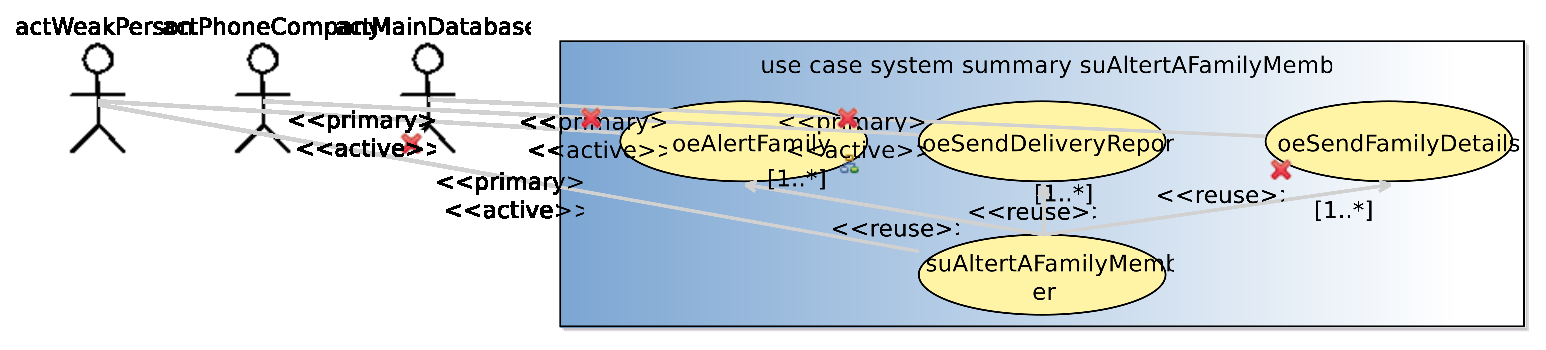
\includegraphics[
angle=0
]{./images-report-gen/usecase-model/summary/uc-suAltertAFamilyMember.eps}
\end{center}
\caption[lu.uni.lassy.excalibur.g01.specification Use Case Diagram: uc-suAltertAFamilyMember]{}
\label{fig:lu.uni.lassy.excalibur.g01.specification-RE-UCD-uc-suAltertAFamilyMember}
\end{figure}
\vspace{0.5cm}

\input{./doc-gen/usecase-model/summary/RE-use-case-suCallSelectedHelpRequest.tex}
\subsubsection{summary-ugRequestHelp}

\label{RE-use-case-ugRequestHelp}



Figure \ref{fig:lu.uni.lassy.excalibur.g01.specification-RE-UCD-uc-ugRequestHelp}
User goal Request help

\begin{figure}[htbp]
\begin{center}

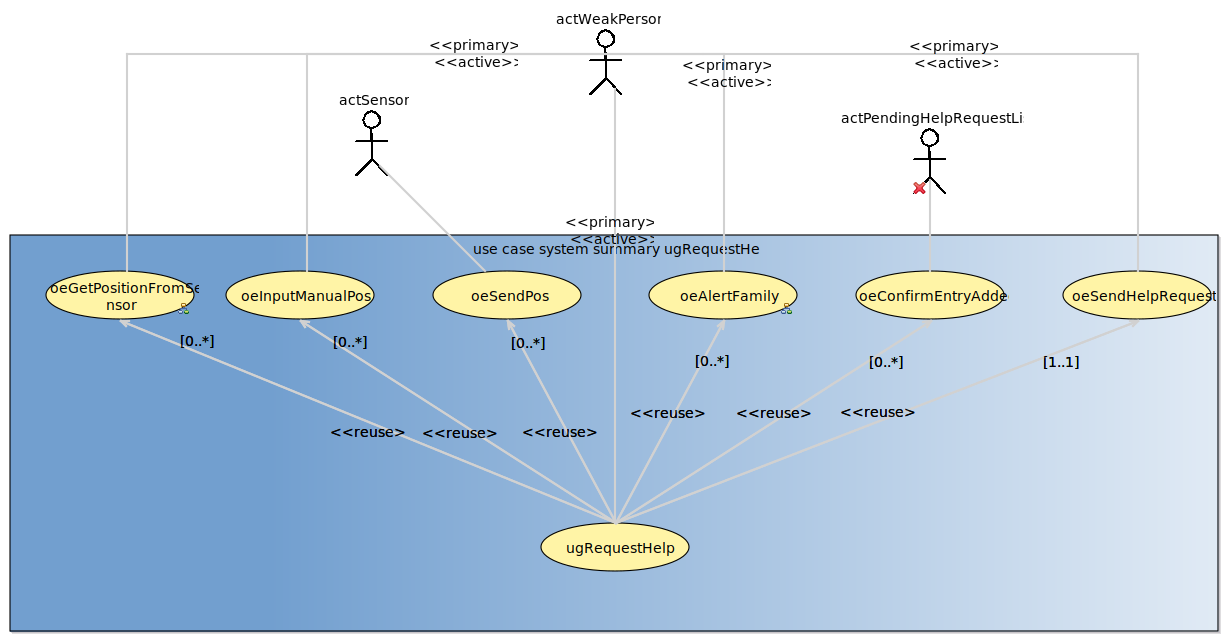
\includegraphics[
angle=0
]{./images-report-gen/usecase-model/summary/uc-ugRequestHelp.eps}
\end{center}
\caption[lu.uni.lassy.excalibur.g01.specification Use Case Diagram: uc-ugRequestHelp]{}
\label{fig:lu.uni.lassy.excalibur.g01.specification-RE-UCD-uc-ugRequestHelp}
\end{figure}
\vspace{0.5cm}



%% ***************************************************************
%% User-Goal Use Cases
\input{./doc-gen/usecase-model/usergoal/RE-use-case-ugAssignPriorityToHelpRequest.tex}
\subsubsection{usergoal-ugGetMissionInRange}

\label{RE-use-case-ugGetMissionInRange}


The actVolunteer's goal is to retrieve help requests that are in a specific range 		  


\begin{usecase}
  \addheading{Use-Case Description}
  \addsingletwocolumnrow{Name}{ugGetMissionInRange}
  \addsingletwocolumnrow{Scope}{system}
  \addsingletwocolumnrow{Level}{usergoal}
  

\addrowheading{Primary actor(s)}
\addnumberedsinglerow{}{\msrcode{actVolunteer[active]}}


\addrowheading{Secondary actor(s)}
\addnumberedsinglerow{}{\msrcode{actPositionRequester[]}}
\addnumberedsinglerow{}{\msrcode{actSensor[]}}

\addrowheading{Goal(s) description}
\addsinglerow{The actVolunteer's goal is to retrieve help requests that are in a specific range }


\addrowheading{Protocol condition(s)}
\addnumberedsinglerow{}{The system has been deployed.
}

\addrowheading{Pre-condition(s)}
\addnumberedsinglerow{}{
}

\addrowheading{Main post-condition(s)}
\addnumberedsinglerow{}{The system returns a non null list of HelpRequest or a message indicating that none has been found within the specified range
}

\addrowheading{Main Steps}
\addalphanumberedsinglerow{}{the actor \msrcode{actPositionRequester} executes the \msrucname{oeGetPositionFromSensor} use case}
\addalphanumberedsinglerow{}{the actor \msrcode{actSensor} executes the \msrucname{oeSendPos} use case}
\addalphanumberedsinglerow{}{the actor \msrcode{actVolunteer} executes the \msrucname{oeGetInRangeMission} use case}

\addrowheading{Additional Information}
\addsinglerow{
none
}

\end{usecase} 


Figure \ref{fig:lu.uni.lassy.excalibur.g01.specification-RE-UCD-uc-ugGetMissionInRange}
User goal Get mission in range

\begin{figure}[htbp]
\begin{center}

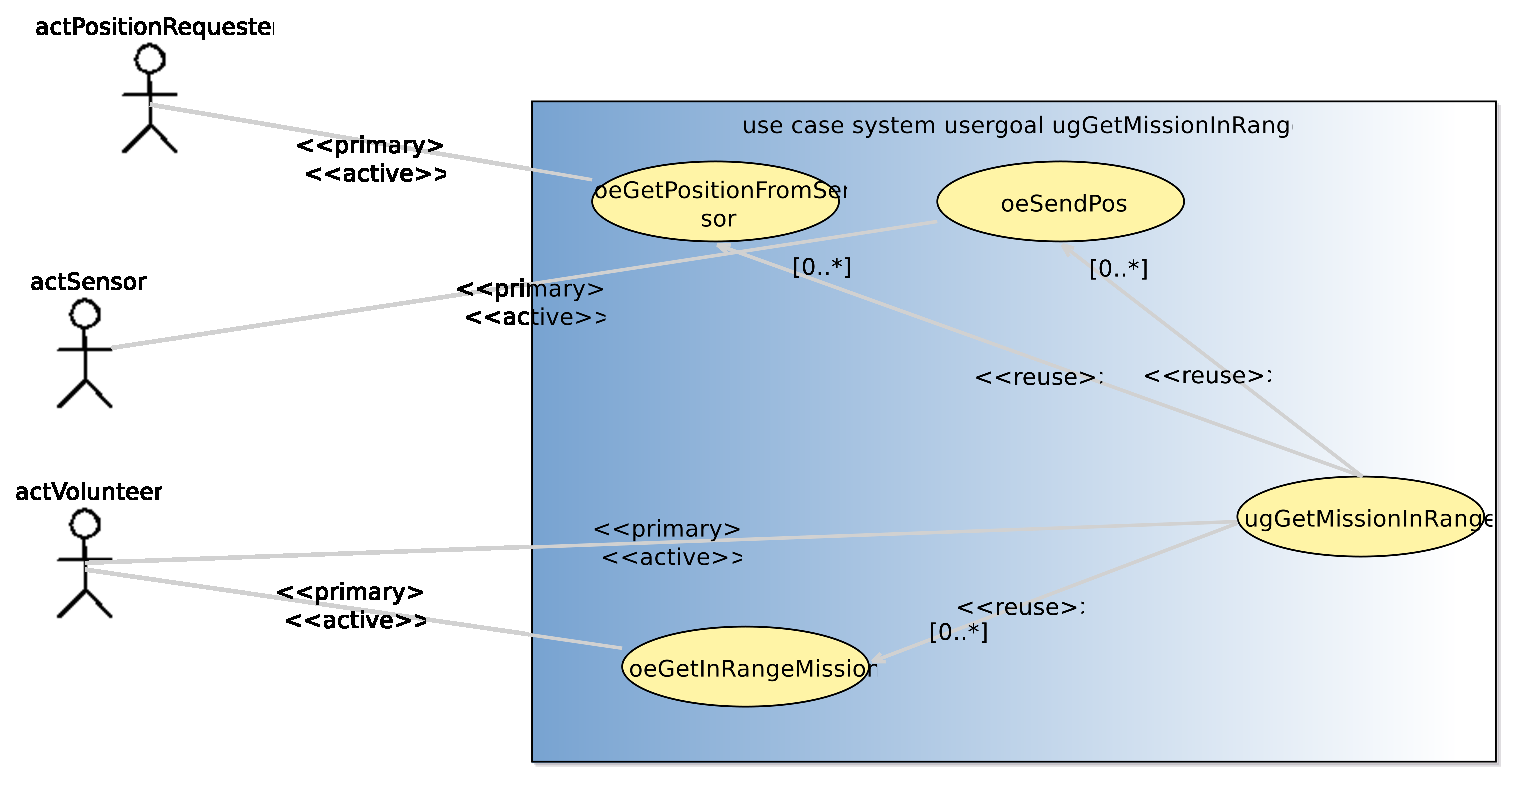
\includegraphics[
angle=0
]{./images-report-gen/usecase-model/usergoal/uc-ugGetMissionInRange.eps}
\end{center}
\caption[lu.uni.lassy.excalibur.g01.specification Use Case Diagram: uc-ugGetMissionInRange]{}
\label{fig:lu.uni.lassy.excalibur.g01.specification-RE-UCD-uc-ugGetMissionInRange}
\end{figure}
\vspace{0.5cm}

\input{./doc-gen/usecase-model/usergoal/RE-use-case-ugRetrievePendingHelpRequestDetails.tex}


%% ***************************************************************
%% Subfunction Use Cases
\subsubsection{subfunction-oeAlertFamily}

\label{RE-use-case-oeAlertFamily}


Figure \ref{fig:lu.uni.lassy.excalibur.g01.specification-RE-UCD-uc-oeAlertFamily}
Sub Function AlertFamily

\begin{figure}[htbp]
\begin{center}

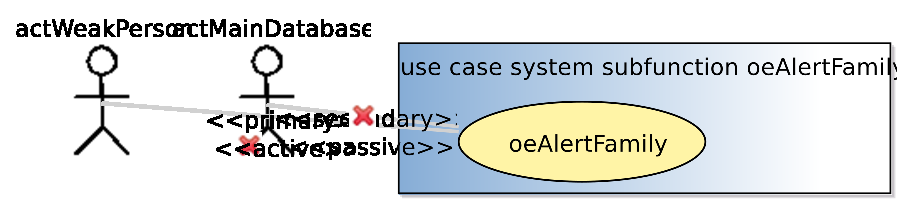
\includegraphics[
angle=0
]{./images-report-gen/usecase-model/subfunction/uc-oeAlertFamily.eps}
\end{center}
\caption[lu.uni.lassy.excalibur.g01.specification Use Case Diagram: uc-oeAlertFamily]{}
\label{fig:lu.uni.lassy.excalibur.g01.specification-RE-UCD-uc-oeAlertFamily}
\end{figure}
\vspace{0.5cm}

\subsubsection{subfunction-oeGetPositionFromSensor}

\label{RE-use-case-oeGetPositionFromSensor}


Figure \ref{fig:lu.uni.lassy.excalibur.g01.specification-RE-UCD-uc-oeGetPositionFromSensor}
 Sub Function Get position from sensor 

\begin{figure}[htbp]
\begin{center}

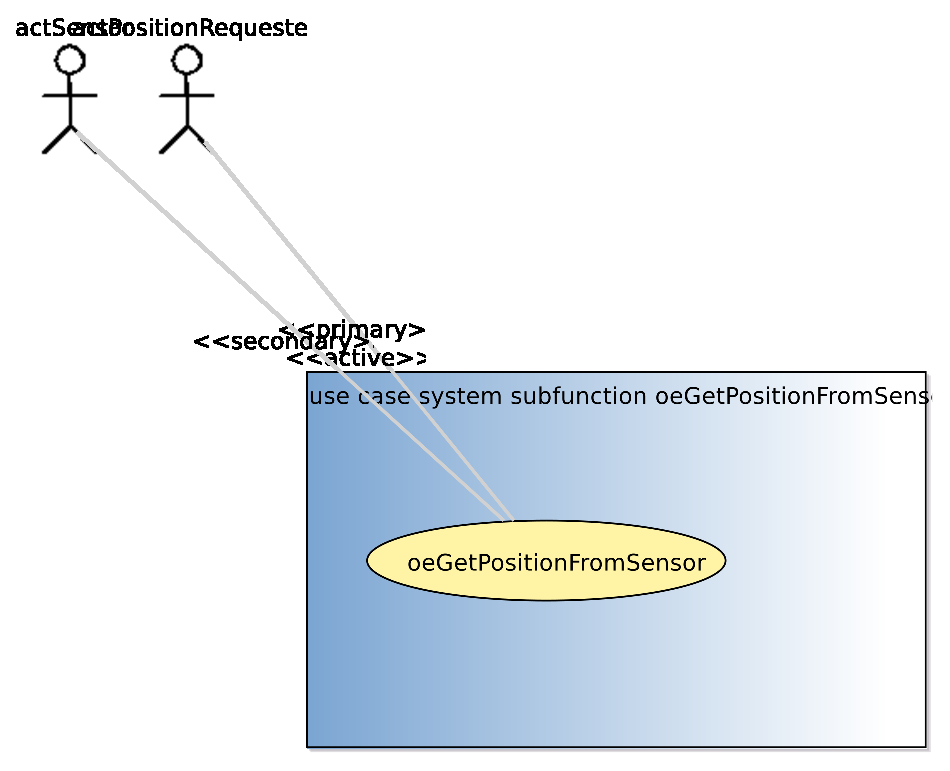
\includegraphics[
angle=0
,scale=0.5
]{./images-report-gen/usecase-model/subfunction/uc-oeGetPositionFromSensor.eps}
\end{center}
\caption[lu.uni.lassy.excalibur.g01.specification Use Case Diagram: uc-oeGetPositionFromSensor]{}
\label{fig:lu.uni.lassy.excalibur.g01.specification-RE-UCD-uc-oeGetPositionFromSensor}
\end{figure}
\vspace{0.5cm}

\subsubsection{subfunction-oeSendFamilyDetails}

\label{RE-use-case-oeSendFamilyDetails}


Figure \ref{fig:lu.uni.lassy.excalibur.g01.specification-RE-UCD-uc-oeSendFamilyDetails}
Sub function Send family details

\begin{figure}[htbp]
\begin{center}

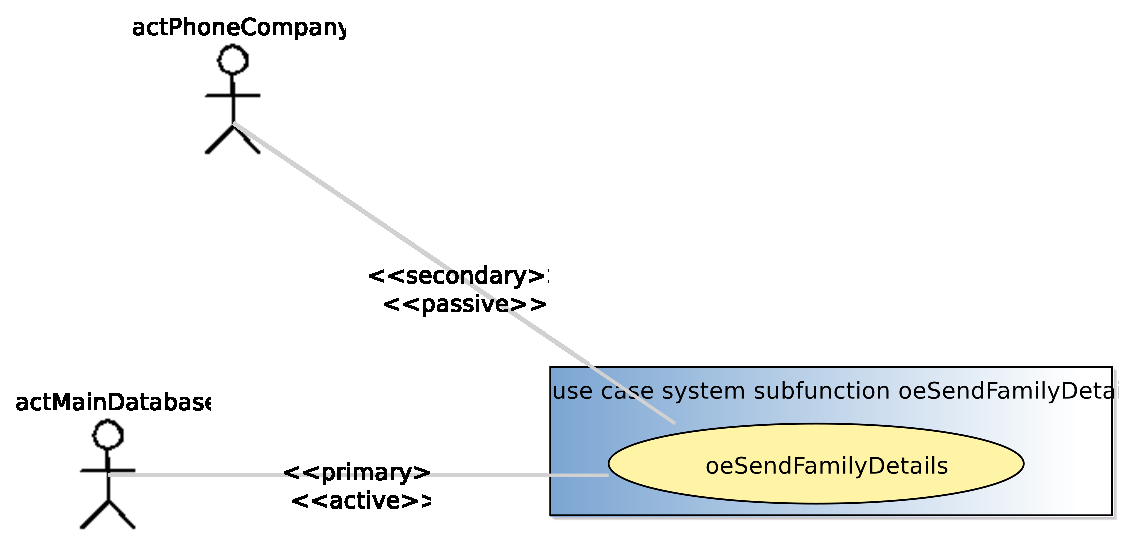
\includegraphics[
angle=0
]{./images-report-gen/usecase-model/subfunction/uc-oeSendFamilyDetails.eps}
\end{center}
\caption[lu.uni.lassy.excalibur.g01.specification Use Case Diagram: uc-oeSendFamilyDetails]{}
\label{fig:lu.uni.lassy.excalibur.g01.specification-RE-UCD-uc-oeSendFamilyDetails}
\end{figure}
\vspace{0.5cm}




%% ***************************************************************
%% Use Case Instances
\pagebreak
\subsection{Use Case Instance(s)}


%% ***************************************************************
%% Summary Use Case Instances

	\subsubsection{Use-Case Instance - uciCallSelectedHelp:suCallSelectedHelpRequest}
	

	
	Figure \ref{fig:lu.uni.lassy.excalibur.g01.specification-RE-UC-uci-uciCallSelectedHelp}
	Call Selected help request
	
	\begin{figure}[htbp]
	\begin{center}
	
	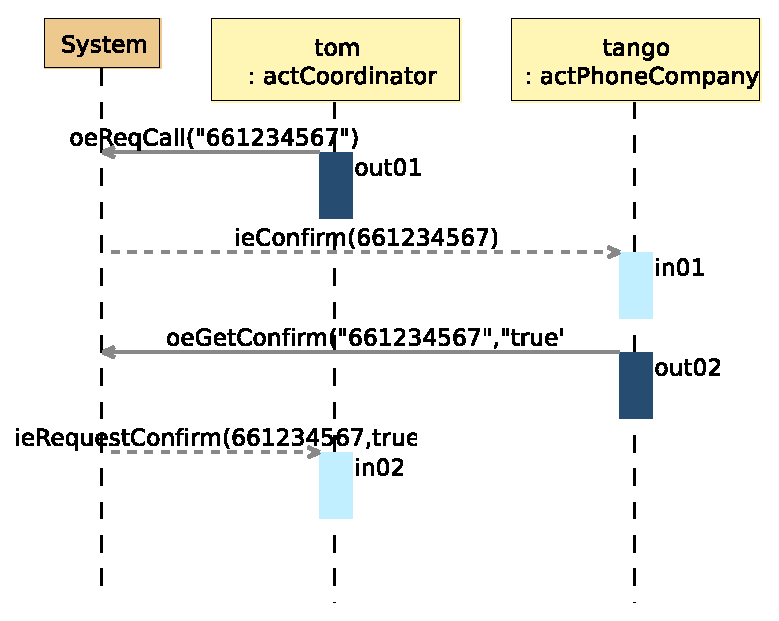
\includegraphics[
	angle=0
	]{./images-report-gen/usecase-model/summary/uci-uciCallSelectedHelp.eps}
	\end{center}
	\caption[lu.uni.lassy.excalibur.g01.specification Sequence Diagram: uci-uciCallSelectedHelp]{}
	\label{fig:lu.uni.lassy.excalibur.g01.specification-RE-UC-uci-uciCallSelectedHelp}
	\end{figure}
	\vspace{0.5cm}


	\subsubsection{Use-Case Instance - uciSendHelpRequest:ugRequestHelp}
	

	
	Figure \ref{fig:lu.uni.lassy.excalibur.g01.specification-RE-UC-uci-uciSendHelpRequest}
	Send help request
	
	\begin{figure}[htbp]
	\begin{center}
	
	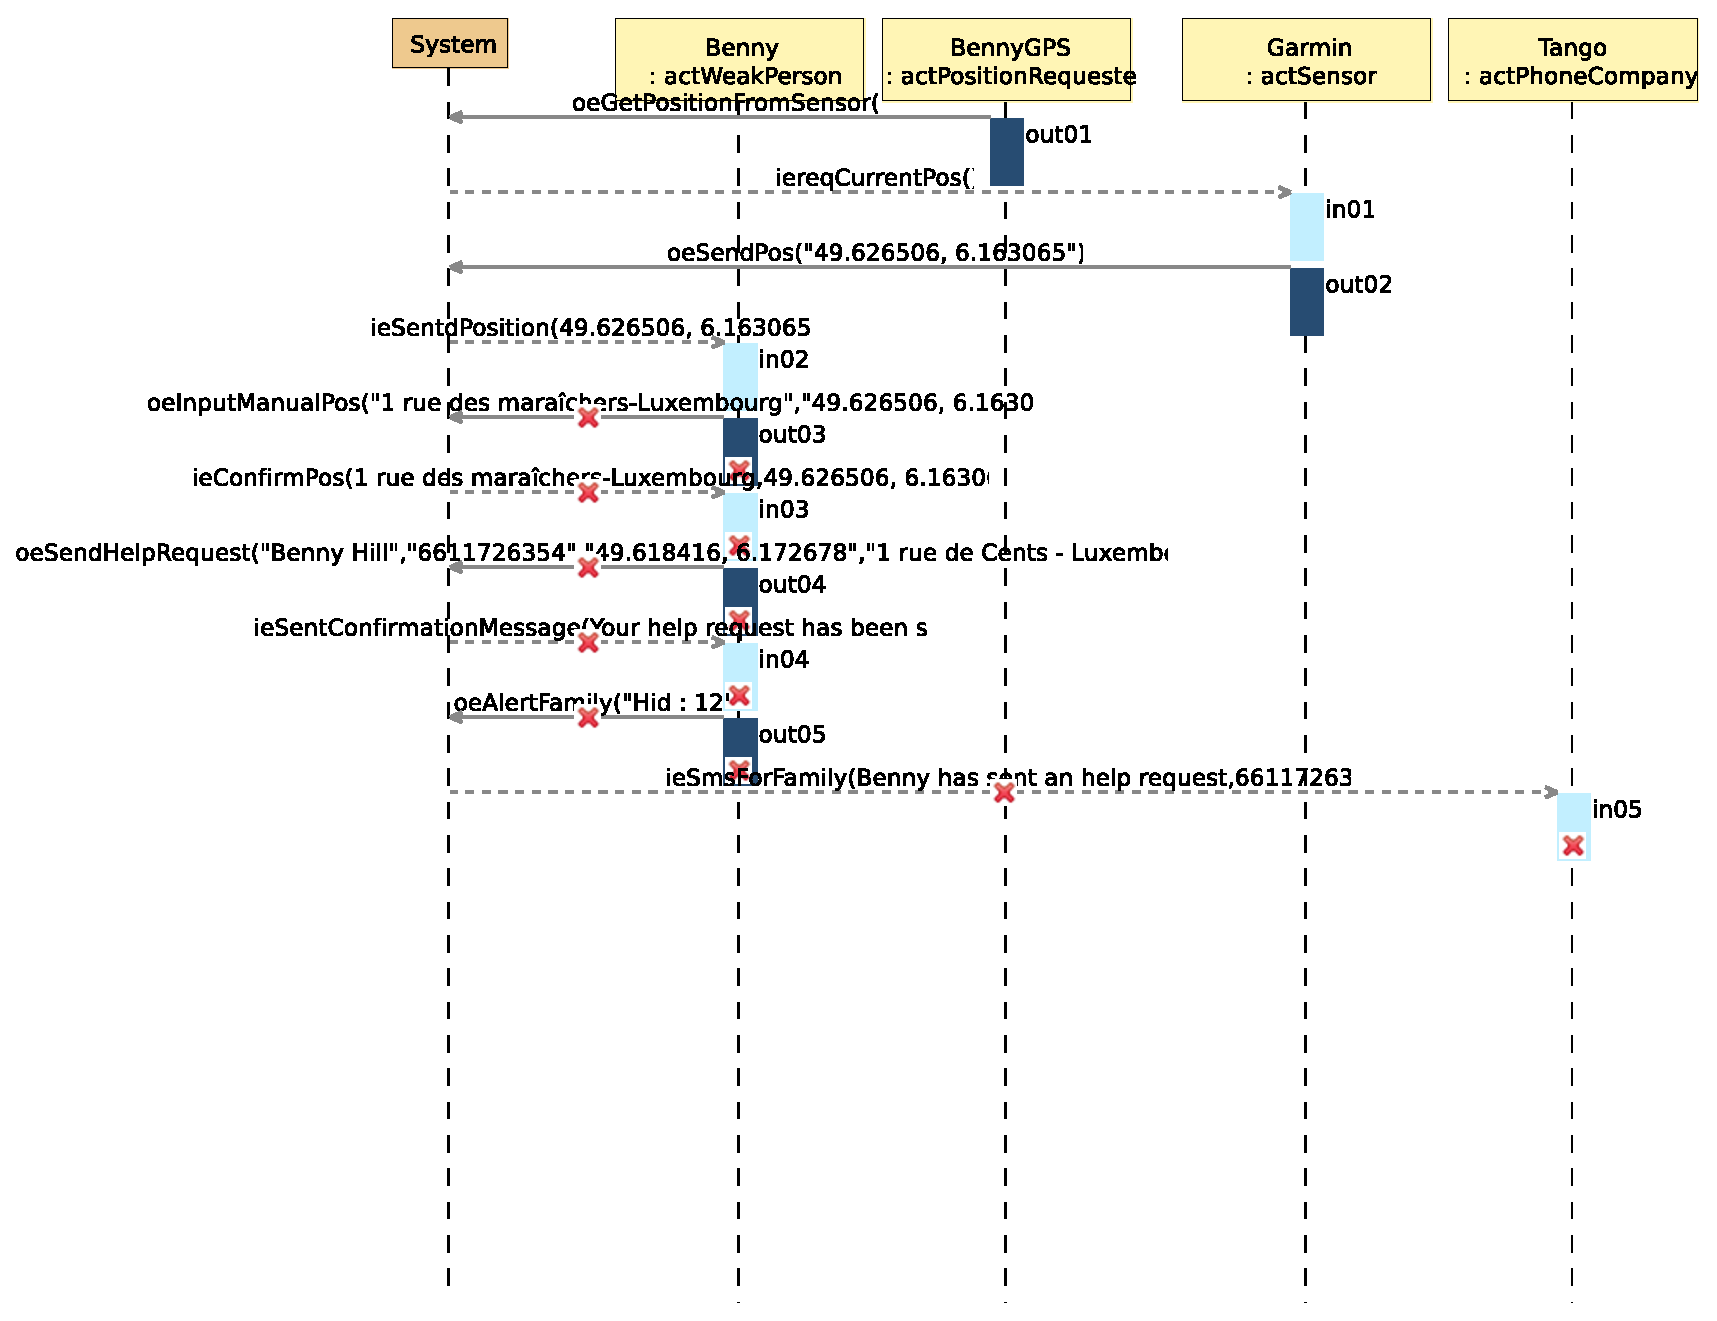
\includegraphics[
	angle=0
	]{./images-report-gen/usecase-model/summary/uci-uciSendHelpRequest.eps}
	\end{center}
	\caption[lu.uni.lassy.excalibur.g01.specification Sequence Diagram: uci-uciSendHelpRequest]{}
	\label{fig:lu.uni.lassy.excalibur.g01.specification-RE-UC-uci-uciSendHelpRequest}
	\end{figure}
	\vspace{0.5cm}




%% ***************************************************************
%% User-Goal Use Case Instances

	\subsubsection{Use-Case Instance - uciGetInRangeMission:ugGetMissionInRange}
	

	
	Figure \ref{fig:lu.uni.lassy.excalibur.g01.specification-RE-UC-uci-uciGetInRangeMission}
	Get in range mission
	
	\begin{figure}[htbp]
	\begin{center}
	
	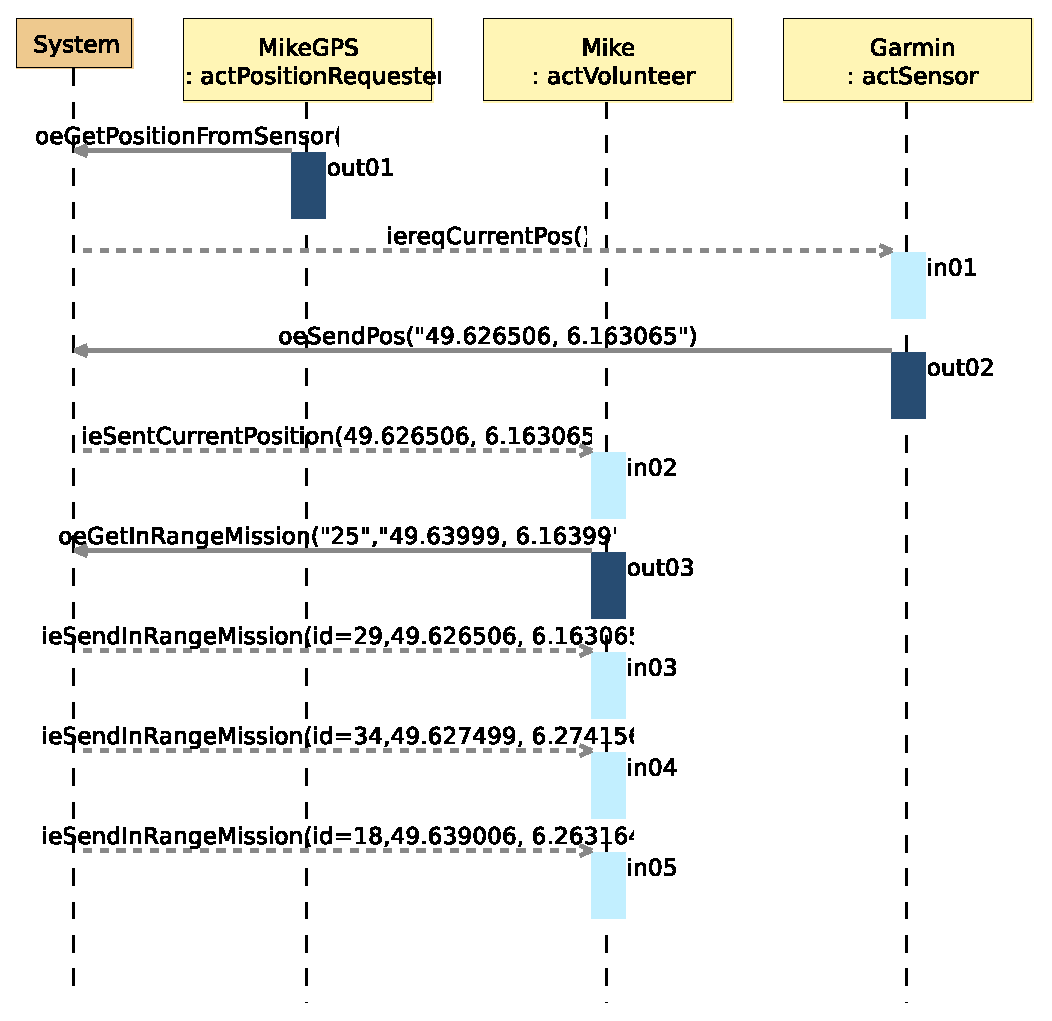
\includegraphics[
	angle=0
	]{./images-report-gen/usecase-model/usergoal/uci-uciGetInRangeMission.eps}
	\end{center}
	\caption[lu.uni.lassy.excalibur.g01.specification Sequence Diagram: uci-uciGetInRangeMission]{}
	\label{fig:lu.uni.lassy.excalibur.g01.specification-RE-UC-uci-uciGetInRangeMission}
	\end{figure}
	\vspace{0.5cm}


	\subsubsection{Use-Case Instance - uciGetPendingHelpRequests:ugRetrievePendingHelpRequestDetails}
	

	
	Figure \ref{fig:lu.uni.lassy.excalibur.g01.specification-RE-UC-uci-uciGetPendingHelpRequests}
	Get pending help requests 
	
	\begin{figure}[htbp]
	\begin{center}
	
	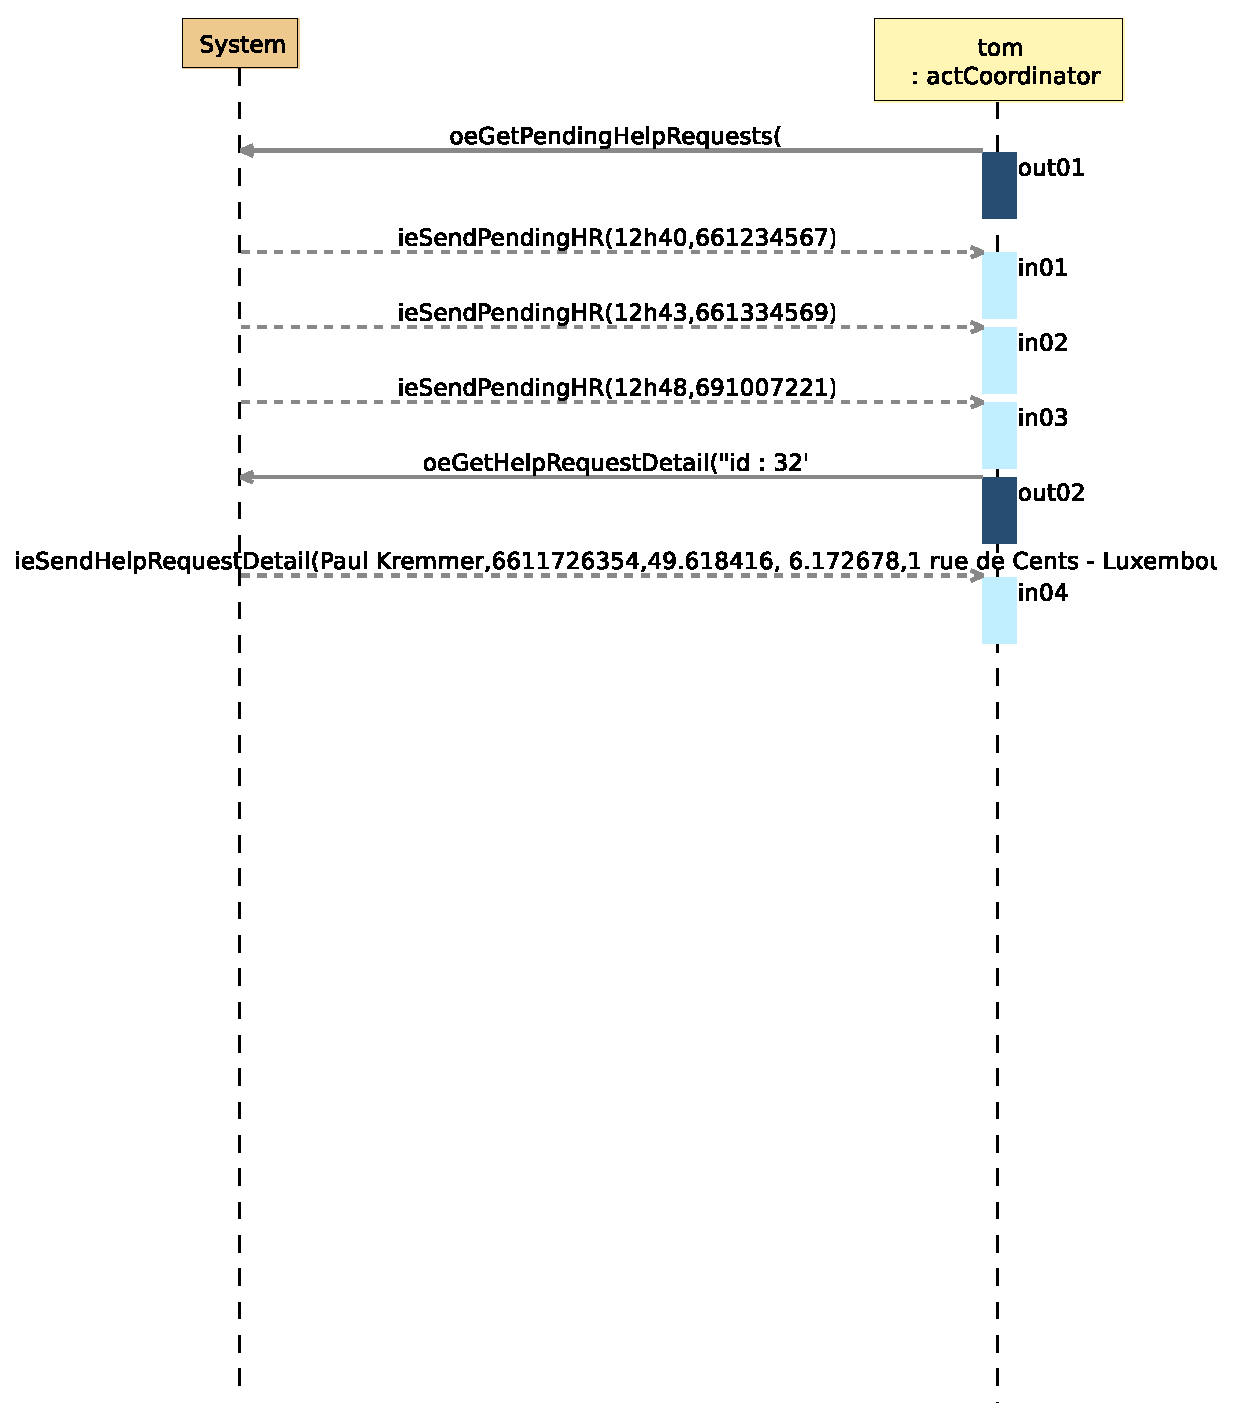
\includegraphics[
	angle=0
	]{./images-report-gen/usecase-model/usergoal/uci-uciGetPendingHelpRequests.eps}
	\end{center}
	\caption[lu.uni.lassy.excalibur.g01.specification Sequence Diagram: uci-uciGetPendingHelpRequests]{}
	\label{fig:lu.uni.lassy.excalibur.g01.specification-RE-UC-uci-uciGetPendingHelpRequests}
	\end{figure}
	\vspace{0.5cm}




%% ***************************************************************
%% Subfunction Use Case Instances


\chapter{Environment Model}
\label{chap:lu.uni.lassy.excalibur.g01.specification-EM}


\section{Environment model view(s)}		
There are no view(s) for the \msrmessir environment model.



\section{Actors and Interfaces Descriptions}
\label{sec:lu.uni.lassy.excalibur.g01.specification-EM-Actors-Descriptions}


		
We provide for the given views the description of the actors together with their associated input and output interface descriptions.
\subsection{\msrcode{actCoordinator} Actor}


\begin{actortable}
	\addheading{Actor}
	
	\adddoublerow{actCoordinator}{Environment Coordinator}
	
	
	
	
	

	\addrowheading{OutputInterfaces}
	\addnumbereddoublerow{OUT}{\hypertarget{actCoordinator.outactCoordinator.oeLogin}
			{\msrcode{oeLogin():ptBoolean}}}
			{}
	\addnumbereddoublerow{OUT}{\hypertarget{actCoordinator.outactCoordinator.oeLogout}
			{\msrcode{oeLogout():ptBoolean}}}
			{}
	\addnumbereddoublerow{OUT}{\hypertarget{actCoordinator.outactCoordinator.oeGetPendingHelpRequests}
			{\msrcode{oeGetPendingHelpRequests():ptBoolean}}}
			{}
	\addnumbereddoublerow{OUT}{\hypertarget{actCoordinator.outactCoordinator.oeGetHelpRequestDetail}
			{\msrcode{oeGetHelpRequestDetail(AdtHelpRequestId:dtHRid):ptBoolean}}}
			{}
	\addnumbereddoublerow{OUT}{\hypertarget{actCoordinator.outactCoordinator.oeProceedCall}
			{\msrcode{oeProceedCall():ptBoolean}}}
			{}
	\addnumbereddoublerow{OUT}{\hypertarget{actCoordinator.outactCoordinator.oeSetRiskLevel}
			{\msrcode{oeSetRiskLevel():ptBoolean}}}
			{}
	\addnumbereddoublerow{OUT}{\hypertarget{actCoordinator.outactCoordinator.oeGetVolunteersList}
			{\msrcode{oeGetVolunteersList():ptBoolean}}}
			{}
	\addnumbereddoublerow{OUT}{\hypertarget{actCoordinator.outactCoordinator.oeReqCall}
			{\msrcode{oeReqCall():ptBoolean}}}
			{}
	\addnumbereddoublerow{OUT}{\hypertarget{actCoordinator.outactCoordinator.oeReqCheckbox}
			{\msrcode{oeReqCheckbox():ptBoolean}}}
			{}
	\addnumbereddoublerow{OUT}{\hypertarget{actCoordinator.outactCoordinator.oeSendFilledCheckbox}
			{\msrcode{oeSendFilledCheckbox():ptBoolean}}}
			{}
	\addnumbereddoublerow{OUT}{\hypertarget{actCoordinator.outactCoordinator.oeConfirmPriority}
			{\msrcode{oeConfirmPriority():ptBoolean}}}
			{}
	
	\addrowheading{InputInterfaces}
	\addnumbereddoublerow{IN}{\msrcode{ieSendPendingHelpRequestList(AdtTime:dtTime, AdtPhoneNumber:dtPhoneNumber):ptBoolean}}
							 {}
	\addnumbereddoublerow{IN}{\msrcode{ieSendHelpRequestDetail(AdtName:dtName, AdtPhoneNumber:dtPhoneNumber, AdtCoordinates:dtCoordinates, AdtAddress:dtAddress):ptBoolean}}
							 {}
	\addnumbereddoublerow{IN}{\msrcode{ieSendVolunteerList():ptBoolean}}
							 {}
	\addnumbereddoublerow{IN}{\msrcode{ieConfirm():ptBoolean}}
							 {}
	\addnumbereddoublerow{IN}{\msrcode{ieSendCheckbox():ptBoolean}}
							 {}
	\addnumbereddoublerow{IN}{\msrcode{ieSendCalculatedPriority():ptBoolean}}
							 {}
	\addnumbereddoublerow{IN}{\msrcode{ieSendResult():ptBoolean}}
							 {}
	
\end{actortable}

\subsection{\msrcode{actMainDatabase} Actor}


\begin{actortable}
	\addheading{Actor}
	
	\adddoublerow{actMainDatabase}{Environment Main Database}
	
	
	
	
	

	\addrowheading{OutputInterfaces}
	\addnumbereddoublerow{OUT}{\hypertarget{actMainDatabase.outactMainDatabase.oeSentPendingHelpRequest}
			{\msrcode{oeSentPendingHelpRequest(AdtTime:dtTime, AdtPhoneNumber:dtPhoneNumber):ptBoolean}}}
			{}
	\addnumbereddoublerow{OUT}{\hypertarget{actMainDatabase.outactMainDatabase.oeSendHRDetails}
			{\msrcode{oeSendHRDetails(AdtName:dtName, AdtPhoneNumber:dtPhoneNumber, AdtCoordinates:dtCoordinates, AdtAddress:dtAddress):ptBoolean}}}
			{}
	\addnumbereddoublerow{OUT}{\hypertarget{actMainDatabase.outactMainDatabase.oeSendFamilyDetails}
			{\msrcode{oeSendFamilyDetails(AdtName:dtName, AdtPhoneNumber:dtPhoneNumber, AdtMessage:dtMessage):ptBoolean}}}
			{}
	\addnumbereddoublerow{OUT}{\hypertarget{actMainDatabase.outactMainDatabase.oeConfirmEntryAdded}
			{\msrcode{oeConfirmEntryAdded(AdtId:dtHRid, AdtConfirmation:ptBoolean):ptBoolean}}}
			{}
	
	\addrowheading{InputInterfaces}
	\addnumbereddoublerow{IN}{\msrcode{ieReqPendingHelpRequests():ptBoolean}}
							 {}
	\addnumbereddoublerow{IN}{\msrcode{ieRequHRDetails(AdtId:dtHRid):ptBoolean}}
							 {}
	\addnumbereddoublerow{IN}{\msrcode{ieSendPendingHR(AdtTime:dtTime):ptBoolean}}
							 {}
	\addnumbereddoublerow{IN}{\msrcode{ieFamilyDetailsRequest():ptBoolean}}
							 {}
	\addnumbereddoublerow{IN}{\msrcode{ieConfirmationOfSmsSend():ptBoolean}}
							 {}
	\addnumbereddoublerow{IN}{\msrcode{ieFamilyDeliveryReport():ptBoolean}}
							 {}
	\addnumbereddoublerow{IN}{\msrcode{ieAddEntry(AdtName:dtName, AdtPhoneNumber:dtPhoneNumber, AdtCoordinates:dtCoordinates, AdtAddress:dtAddress):ptBoolean}}
							 {}
	
\end{actortable}

\subsection{\msrcode{actPhoneCompany} Actor}


\begin{actortable}
	\addheading{Actor}
	
	\adddoublerow{actPhoneCompany}{Env Phone company }
	
	
	
	
	

	\addrowheading{OutputInterfaces}
	\addnumbereddoublerow{OUT}{\hypertarget{actPhoneCompany.outactPhoneCompany.oeGetConfirm}
			{\msrcode{oeGetConfirm():ptBoolean}}}
			{}
	\addnumbereddoublerow{OUT}{\hypertarget{actPhoneCompany.outactPhoneCompany.oeGetDeliveryReport}
			{\msrcode{oeGetDeliveryReport():ptBoolean}}}
			{}
	
	\addrowheading{InputInterfaces}
	\addnumbereddoublerow{IN}{\msrcode{ieRequestConfirm(AdtPhoneNumber:dtPhoneNumber):ptBoolean}}
							 {}
	\addnumbereddoublerow{IN}{\msrcode{ieSmsForFamily(AdtPhoneNumber:dtPhoneNumber, AdtMessage:dtMessage):ptBoolean}}
							 {}
	
\end{actortable}

\subsection{\msrcode{actPositionInputActor} Actor}


\begin{actortable}
	\addheading{Actor}
	
	\adddoublerow{actPositionInputActor}{Env PositionInputActor}
	
	
	
	
	

	\addrowheading{OutputInterfaces}
	\addnumbereddoublerow{OUT}{\hypertarget{actPositionInputActor.outactPositionInputActor.oeInputPost}
			{\msrcode{oeInputPost():ptBoolean}}}
			{}
	
	\addrowheading{InputInterfaces}
	\addnumbereddoublerow{IN}{\msrcode{ieSentPosition():ptBoolean}}
							 {}
	
\end{actortable}

\subsection{\msrcode{actPositionRequester} Actor}


\begin{actortable}
	\addheading{Actor}
	
	\adddoublerow{actPositionRequester}{Env PositionRequester}
	
	
	
	
	

	\addrowheading{OutputInterfaces}
	\addnumbereddoublerow{OUT}{\hypertarget{actPositionRequester.outactPositionRequester.oeGetPositionFromSensor}
			{\msrcode{oeGetPositionFromSensor():ptBoolean}}}
			{}
	
	\addrowheading{InputInterfaces}
	\addnumbereddoublerow{IN}{\msrcode{ieSendSensorPosition():ptBoolean}}
							 {}
	
\end{actortable}

\subsection{\msrcode{actSensor} Actor}


\begin{actortable}
	\addheading{Actor}
	
	\adddoublerow{actSensor}{Env Sensor}
	
	
	
	
	

	\addrowheading{OutputInterfaces}
	\addnumbereddoublerow{OUT}{\hypertarget{actSensor.outactSensor.oeSendPos}
			{\msrcode{oeSendPos():ptBoolean}}}
			{}
	
	\addrowheading{InputInterfaces}
	\addnumbereddoublerow{IN}{\msrcode{iereqCurrentPos():ptBoolean}}
							 {}
	
\end{actortable}

\subsection{\msrcode{actVolunteer} Actor}


\begin{actortable}
	\addheading{Actor}
	
	\adddoublerow{actVolunteer}{Env Volunteer}
	
	
	
	
	

	\addrowheading{OutputInterfaces}
	\addnumbereddoublerow{OUT}{\hypertarget{actVolunteer.outactVolunteer.oeLogin}
			{\msrcode{oeLogin():ptBoolean}}}
			{}
	\addnumbereddoublerow{OUT}{\hypertarget{actVolunteer.outactVolunteer.oeLogout}
			{\msrcode{oeLogout():ptBoolean}}}
			{}
	\addnumbereddoublerow{OUT}{\hypertarget{actVolunteer.outactVolunteer.oeGetPosition}
			{\msrcode{oeGetPosition():ptBoolean}}}
			{}
	\addnumbereddoublerow{OUT}{\hypertarget{actVolunteer.outactVolunteer.oeGetMissionInRagne}
			{\msrcode{oeGetMissionInRagne(AdtRange:dtRange, AdtPosition:dtCoordinates):ptBoolean}}}
			{}
	\addnumbereddoublerow{OUT}{\hypertarget{actVolunteer.outactVolunteer.oeAcceptMission}
			{\msrcode{oeAcceptMission(AdtId:dtHRid):ptBoolean}}}
			{}
	
	\addrowheading{InputInterfaces}
	\addnumbereddoublerow{IN}{\msrcode{ieSentCurrentPosition(AdtCoordinates:dtCoordinates):ptBoolean}}
							 {}
	\addnumbereddoublerow{IN}{\msrcode{ieSentMissionConfirmation():ptBoolean}}
							 {}
	\addnumbereddoublerow{IN}{\msrcode{ieSendRange():ptBoolean}}
							 {}
	\addnumbereddoublerow{IN}{\msrcode{ieSendInRangeMission(AdtId:dtHRid, AdtCoordinates:dtCoordinates):ptBoolean}}
							 {}
	
\end{actortable}

\subsection{\msrcode{actWeakPerson} Actor}


\begin{actortable}
	\addheading{Actor}
	
	\adddoublerow{actWeakPerson}{Env WeakPerson}
	
	
	
	
	

	\addrowheading{OutputInterfaces}
	\addnumbereddoublerow{OUT}{\hypertarget{actWeakPerson.outactWeakPerson.oeSendHelpRequest}
			{\msrcode{oeSendHelpRequest():ptBoolean}}}
			{}
	\addnumbereddoublerow{OUT}{\hypertarget{actWeakPerson.outactWeakPerson.oeLogin}
			{\msrcode{oeLogin():ptBoolean}}}
			{}
	\addnumbereddoublerow{OUT}{\hypertarget{actWeakPerson.outactWeakPerson.oeLogout}
			{\msrcode{oeLogout():ptBoolean}}}
			{}
	\addnumbereddoublerow{OUT}{\hypertarget{actWeakPerson.outactWeakPerson.oeGetpostition}
			{\msrcode{oeGetpostition():ptBoolean}}}
			{}
	\addnumbereddoublerow{OUT}{\hypertarget{actWeakPerson.outactWeakPerson.oeInputManualPos}
			{\msrcode{oeInputManualPos():ptBoolean}}}
			{}
	\addnumbereddoublerow{OUT}{\hypertarget{actWeakPerson.outactWeakPerson.oeGetInfo}
			{\msrcode{oeGetInfo():ptBoolean}}}
			{}
	\addnumbereddoublerow{OUT}{\hypertarget{actWeakPerson.outactWeakPerson.oeGetPositionFromSensor}
			{\msrcode{oeGetPositionFromSensor():ptBoolean}}}
			{}
	\addnumbereddoublerow{OUT}{\hypertarget{actWeakPerson.outactWeakPerson.oeAlertFamily}
			{\msrcode{oeAlertFamily():ptBoolean}}}
			{}
	
	\addrowheading{InputInterfaces}
	\addnumbereddoublerow{IN}{\msrcode{ieSentdPosition():ptBoolean}}
							 {}
	\addnumbereddoublerow{IN}{\msrcode{ieSentConfirmationMessage():ptBoolean}}
							 {}
	\addnumbereddoublerow{IN}{\msrcode{ieSendInfo():ptBoolean}}
							 {}
	\addnumbereddoublerow{IN}{\msrcode{ieConfirmPos():ptBoolean}}
							 {}
	
\end{actortable}

\subsection{\msrcode{actWeakPersonFamily} Actor}


\begin{actortable}
	\addheading{Actor}
	
	\adddoublerow{actWeakPersonFamily}{Env WeakPersonFamily}
	
	
	
	
	

	\addrowheading{OutputInterfaces}
	\addnumbereddoublerow{OUT}{\hypertarget{actWeakPersonFamily.outactWeakPersonFamily.oeSubscribe}
			{\msrcode{oeSubscribe():ptBoolean}}}
			{}
	\addnumbereddoublerow{OUT}{\hypertarget{actWeakPersonFamily.outactWeakPersonFamily.oeConfirmMessage}
			{\msrcode{oeConfirmMessage():ptBoolean}}}
			{}
	\addnumbereddoublerow{OUT}{\hypertarget{actWeakPersonFamily.outactWeakPersonFamily.oeConfirmCall}
			{\msrcode{oeConfirmCall():ptBoolean}}}
			{}
	
	\addrowheading{InputInterfaces}
	\addnumbereddoublerow{IN}{\msrcode{ieSentPosition():ptBoolean}}
							 {}
	\addnumbereddoublerow{IN}{\msrcode{ieGetMessage():ptBoolean}}
							 {}
	\addnumbereddoublerow{IN}{\msrcode{ieGetCall():ptBoolean}}
							 {}
	
\end{actortable}




\chapter{Concept Model}
\label{chap:lu.uni.lassy.excalibur.g01.specification-CM}

\section{Concept Model view(s)}		
There are no view(s) for the \msrmessir concept model.











\section{Concept Model Types Descriptions}
This section provides the textual descriptions of all the types defined in the concept model and that can be part of the graphical views provided.

\subsection{Primary types - Class types descriptions}




The table below is providing comments on the graphical views given for the class types of the primary types. Type logical operations are precisely specified in the operation model.

\begin{datadictionary}
\addheading{Classes}

\adddoublerow{ctCoordinator}{This represent the human that will handle help requests}
\addsingletwocolumnrow{extends}{lu.uni.lassy.excalibur.g01.specification.concepts.primarytypes.classes.ctHuman}
\adddoubletwocolumnrow{attribute}{\msrcode{cId: ptInteger}}{}
\adddoubletwocolumnrow{operation}{\msrcode{init(AcId:dtInteger, Aname:dtName, APhone:dtPhoneNumber, ACoordinates:dtCoordinates, AUsername:dtUserName, APassword:dtPassword):ptBoolean}}{ }
\adddoubletwocolumnrow{operation}{\msrcode{is():ptBoolean}}{ }
\adddoublerow{ctHelpRequest}{This represent the object created by a WeakPErson when asking for help, it is hence associated to exactly 1 human type Weak Person}
\adddoubletwocolumnrow{attribute}{\msrcode{HrTime: dtTime}}{}
\adddoubletwocolumnrow{operation}{\msrcode{init(AHrTime:dtTime):ptBoolean}}{ }
\adddoubletwocolumnrow{operation}{\msrcode{is():ptBoolean}}{ }
\adddoublerow{ctHuman}{Used to define common properties that are shared among other human type }
\adddoubletwocolumnrow{attribute}{\msrcode{coordinates: dtCoordinates}}{}
\adddoubletwocolumnrow{attribute}{\msrcode{name: dtName}}{}
\adddoubletwocolumnrow{attribute}{\msrcode{password: ptString}}{}
\adddoubletwocolumnrow{attribute}{\msrcode{phone: dtPhoneNumber}}{}
\adddoubletwocolumnrow{attribute}{\msrcode{username: ptString}}{}
\adddoubletwocolumnrow{operation}{\msrcode{init(Aname:dtName, APhone:dtPhoneNumber, ACoordinates:dtCoordinates, AUsername:dtUserName, APassword:dtPassword):ptBoolean}}{ }
\adddoubletwocolumnrow{operation}{\msrcode{is():ptBoolean}}{}
\adddoublerow{ctPendingHelpRequest}{This is represent the class type containing 1 or more help request objects}
\adddoubletwocolumnrow{attribute}{\msrcode{listId: ptInteger}}{}
\adddoubletwocolumnrow{operation}{\msrcode{init(AlistId:dtInteger):ptBoolean}}{ }
\adddoubletwocolumnrow{operation}{\msrcode{is():ptBoolean}}{ }
\adddoublerow{ctVolunteer}{This represent the the Human which have the ability to help a weakPerson and look for help requests around him}
\addsingletwocolumnrow{extends}{lu.uni.lassy.excalibur.g01.specification.concepts.primarytypes.classes.ctHuman}
\adddoubletwocolumnrow{attribute}{\msrcode{disp: dtDispo}}{}
\adddoubletwocolumnrow{attribute}{\msrcode{vId: ptInteger}}{}
\adddoubletwocolumnrow{operation}{\msrcode{init(AvId:dtInteger, Adisp:dtDispo, Aname:dtName, APhone:dtPhoneNumber, ACoordinates:dtCoordinates, AUsername:dtUserName, APassword:dtPassword):ptBoolean}}{ }
\adddoubletwocolumnrow{operation}{\msrcode{is():ptBoolean}}{}
\adddoublerow{ctWeakPerson}{This represent the Human who creates help requests}
\addsingletwocolumnrow{extends}{lu.uni.lassy.excalibur.g01.specification.concepts.primarytypes.classes.ctHuman}
\adddoubletwocolumnrow{attribute}{\msrcode{hrId: dtHRid}}{}
\adddoubletwocolumnrow{operation}{\msrcode{init(AWid:dtInteger, Aname:dtName, APhone:dtPhoneNumber, ACoordinates:dtCoordinates, AUsername:dtUserName, APassword:dtPassword):ptBoolean}}{ }
\adddoubletwocolumnrow{operation}{\msrcode{is():ptBoolean}}{}
\end{datadictionary}

\subsection{Primary types - Datatypes types descriptions}



There are no elements in this category in the system analysed.



\subsection{Primary types - Association types descriptions}



There are no association types for the primary types.


\subsection{Primary types - Aggregation types descriptions}


There are no aggregation types for the primary types.


\subsubsection{Primary types - Composition types descriptions}



There are no composition types for the primary types.


\subsection{Secondary types - Class types descriptions}



There are no elements in this category in the system analysed.
		

\subsection{Secondary types - Datatypes types descriptions}



There are no elements in this category in the system analysed.



\subsection{Secondary types - Association types descriptions}



There are no association types for the secondary types.



\subsection{Secondary types - Aggregation types descriptions}



There are no aggregation types for the secondary types.



\subsection{Secondary types - Composition types descriptions}



There are no composition types for the secondary types.





\chapter{Operation Model}
\label{chap:lu.uni.lassy.excalibur.g01.specification-OM}

This section contains the operation schemes of each operation defined in either an actor, its output interface, in a primary or secondary type (class, datatype or enumeration types). 
The \msrmessir OCL code listing is joined to the comment table.

\lstset{
float,
basicstyle=\scriptsize,
language=Messir,
breakatwhitespace=false,
tabsize=2,
breaklines=true,
numbers=left,
emptylines=1,
numbersep=5pt,
showspaces=false,
showstringspaces=false,
showtabs=false
} 


%% ***************************************************************
%% operations for: Environment-Out Interface Operation Schemes

\section{Environment - Out Interface Operation Schemes}
There are no elements in this category in the system analysed.
		

%% ***************************************************************
%% operations for: Environment-Actor Operation Schemes

\section{Environment - Actor Operation Schemes}
There are no elements in this category in the system analysed.
		

%% ***************************************************************
%% operations for primary type classes

\section{Primary Types - Operation Schemes for Classes}
There are no elements in this category in the system analysed.



%% ***************************************************************
%% operations for primary type datatypes and enumerations

\section{Primary Types - Operation Schemes for Datatypes}
There are no elements in this category in the system analysed.




\section{Primary Types - Operation Schemes for Enumerations}
There are no elements in this category in the system analysed.





%% ***************************************************************
%% operations for secondary type classes


\section{Secondary Types - Operation Schemes for Classes}
There are no elements in this category in the system analysed.




%% ***************************************************************
%% operations for secondary type datatypes and enumerations

\section{Secondary Types - Operation Schemes for Datatypes}
There are no elements in this category in the system analysed.



\section{Secondary Types - Operation Schemes for Enumerations}
There are no elements in this category in the system analysed.





\lstset{
float,
basicstyle=\scriptsize,
language=Messir,
breakatwhitespace=false,
tabsize=2,
breaklines=true,
numbers=left,
emptylines=1,
numbersep=5pt,
showspaces=false,
showstringspaces=false,
showtabs=false
} 

\chapter{Test Model(s)}
\label{chap:lu.uni.lassy.excalibur.g01.specification-TM}

There are no elements in this category in the system analysed.








\newpage

% Last Modification:
% @author AUTHOR_NAME
% @date TODAY_DATE


\chapter{Additional Constraints}
\label{chap:additional_constraints}
\newpage

%APPENDICES
\appendix
% Last Modification:
% @author AUTHOR_NAME
% @date TODAY_DATE



% doc-gen

% This is automatically generated and will be overwritten by the Generate Latex.
\newpage

%GLOSSARY
\printglossaries
\newpage


%BIBLIOGRAPHY
\cleardoublepage
\bibliographystyle{./../lu.uni.lassy.excalibur.standard.report.libraries/styles/lncs} 
\bibliography{./../lu.uni.lassy.excalibur.standard.report.libraries/defs/references/messir,doc/bibliography/report}
\label{sec:references}
 
\end{document}
